\documentclass[handout,10pt]{beamer}
\usepackage{mycommands,fancyvrb,outlines,pbox}
\usepackage[round]{natbib}
\usepackage{hyperref} % link references
\usepackage[font=footnotesize]{caption} % caption options
\usepackage{fancyvrb}

\usepackage[tikz]{bclogo}
\presetkeys{bclogo}{
ombre=true,
epBord=3,
couleur = white,
couleurBord = black,
arrondi = 0.2,
logo=\bctrombone
}{}

\definecolor{UniBlue}{RGB}{83,121,170}
\setbeamercolor{title}{fg=UniBlue}
\setbeamercolor{frametitle}{fg=UniBlue}
\newcommand{\coluit}{\color{UniBlue}\it}
\newcommand{\colubf}{\color{UniBlue}\bf}

\DeclareMathOperator*{\diag}{diag}
\DeclareMathOperator*{\Tr}{Tr}
\DeclareMathOperator*{\argmin}{argmin}

% Row color change in table
\makeatletter
\def\zapcolorreset{\let\reset@color\relax\ignorespaces}
\def\colorrows#1{\noalign{\aftergroup\zapcolorreset#1}\ignorespaces}
\makeatother

     \setbeamertemplate{footline}
        {
      \leavevmode%
      \hbox{%
      \begin{beamercolorbox}[wd=.333333\paperwidth,ht=2.25ex,dp=1ex,center]{author in head/foot}%
        \usebeamerfont{author in head/foot}\insertshortauthor~~
        %(\insertshortinstitute)
      \end{beamercolorbox}%
      \begin{beamercolorbox}[wd=.333333\paperwidth,ht=2.25ex,dp=1ex,center]{title in head/foot}%
        \usebeamerfont{title in head/foot}\insertshorttitle
      \end{beamercolorbox}%
      \begin{beamercolorbox}[wd=.333333\paperwidth,ht=2.25ex,dp=1ex,right]{date in head/foot}%
        \usebeamerfont{date in head/foot}\insertshortdate{}\hspace*{2em}

    %#turning the next line into a comment, erases the frame numbers
        %\insertframenumber{} / \inserttotalframenumber\hspace*{2ex} 

      \end{beamercolorbox}}}%

%\def\logo{%
%{\includegraphics[height=1cm]{goldy1.png}}
%}
%%
%\setbeamertemplate{footline}
%{%
%	\hspace*{.05cm}\logo
%  \begin{beamercolorbox}[sep=1em,wd=10cm,rightskip=0.5cm]
%  {footlinecolor,author in head/foot}
%%    \usebeamercolor{UniBlue}
%    \vspace{0.1cm}
%    \insertshortdate \hfill \insertshorttitle
%    \newline
%    \insertshortauthor   - \insertshortinstitute
%    \hfill
%    \hfill \insertframenumber/\inserttotalframenumber
%  \end{beamercolorbox}
%  \vspace*{0.05cm}
%}

%% smart verbatim
\fvset{framesep=1cm,fontfamily=courier,fontsize=\scriptsize,framerule=.3mm,numbersep=1mm,commandchars=\\\{\}}


\title[Your Short Title]{Selection of causal SNPs in Twin Studies data from multi-SNP mixed models}
\author{Subho Majumdar}
%\institute{Where You're From}
%\date{Date of Presentation}

\begin{document}

\begin{frame}
  \titlepage
\end{frame}

% Uncomment these lines for an automatically generated outline.
%\begin{frame}{Outline}
%  \tableofcontents
%\end{frame}

%\begin{frame}{Objective}
%
%\begin{itemize}
%  \item Most GWAS using family-based designs focus on single-SNP analysis to do association analysis;
%  \item The reason is the difficulty to do association tests for individual SNPs in a multiple-SNP linear mixed model;
%  \item Our objective is to take a variable selection approach while remaining within the mixed model sructure;
%  \item We shall utilize a frugal model selection method to identify SNPs with possible association with the quantitative trait in question.
%\end{itemize}
%
%\end{frame}

\begin{frame}{The model}

\begin{itemize}
\item $m$ pedigrees, $i^\text{th}$ pedigree has $n_i$ indivuduals.
\item $y_{ij} = $ measured phenotype in $j$-th individual of $i$-th pedigree.

\end{itemize}

%
\begin{align}\label{eqn:LMMeqn}
\bfY_i = \alpha + \bfG_i \bfbeta + \bfC_i \bfbeta_c + \bfepsilon_i
\end{align}
%
%
\begin{align}\label{eqn:partsOfV}
\bfV_i = \sigma_a^2 \bfPhi_i + \sigma_c^2 {\bf 1} {\bf 1}^T + \sigma_e^2 \bfI_{n_i}
\end{align}
%

where $\bfPhi_i$ is the known relationship matrix = twice the kinship matrix, and $\sigma_a^2, \sigma_c^2, \sigma_e^2$ are the variances corresponding to polygenic effext outside the group of SNPs modeled, shared environment and random error, respectively.
\end{frame}

\begin{frame}{Objective}
Want to detect the non-zero entries of $\bfbeta_g$ in the above model.

State-of-the-art is to perform single-SNP analysis (e.g. using RFGLS) and then correct for multiple correlation. This loses power. We want to use a new bootstrap-based method of \textbf{$e$-values} to improve that.
\end{frame}

\begin{frame}{The $e$-values method}

\begin{enumerate}
\item Estimate the full model coefficient, say $\hat \bfbeta_g$ (by \texttt{regress} etc.)

\item Obtain its bootstrap distribution: $[\hat \bfbeta]$;

\item Replace the $j$-th coefficient with 0, name it $\hat \bfbeta_{-j}$. Do the same for its bootstrap distribution, say $[\hat \bfbeta_{-j}]$. Repeat for all $j$;

\item $e$-value of $j$-th covariate = tail probability of the $q$-th quantile of $E([\hat \bfbeta_{-j}])$ with respect to $E([\hat \bfbeta])$, where $E(.)$ is an \textit{evaluation function};

\item Select $j$-th covariate if $e$-value is less than $qt$-th quantile of $E([\hat \bfbeta])$.
\end{enumerate}
\end{frame}

\begin{frame}{Simulation setup}
\begin{itemize}
\item 250 pedigrees, each of size 4: consisting of parents and MZ twins;
\item $\alpha = 0$, no environmental covariates;
\item 50 SNPs in correlated blocks of 6,4,6,4 and 30: MAF of SNPs in the blocks 0.2, 0.4, 0.4, 0.25 and 0.25;
\item $\sigma^2_a = 4, \sigma^2_c = 1, \sigma^2_e = 1$;
\item First SNP of first 4 blocks are causal: each having heritability $h\%$\\

\item Full setup replicated 100 times.
\end{itemize}
\end{frame}

\begin{frame}
\begin{figure}
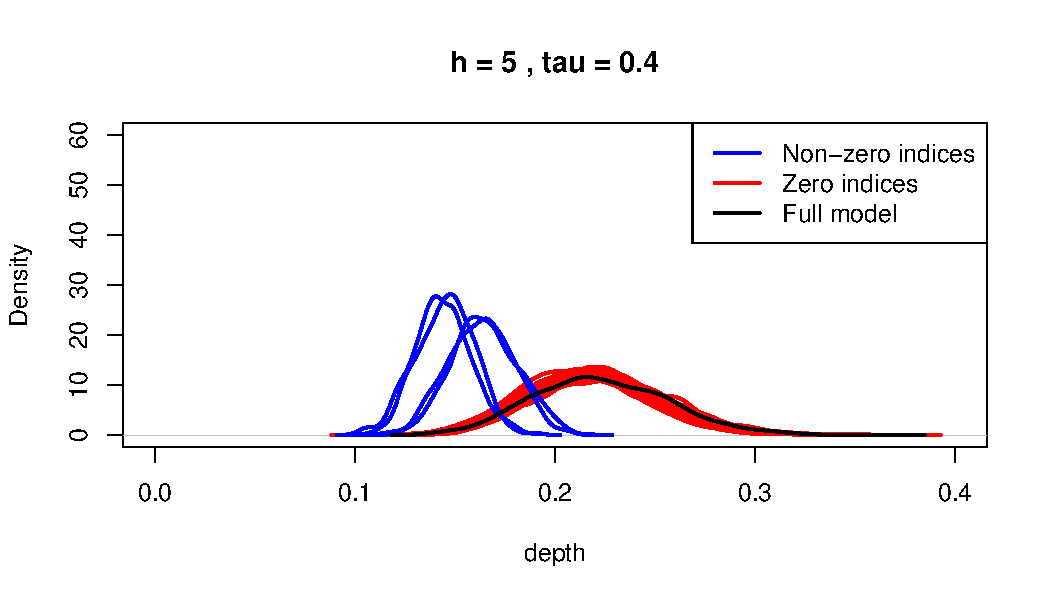
\includegraphics[width=\textwidth]{../Codes/plot_h5_tau4}
\end{figure}
\end{frame}

\begin{frame}{Simulation results}
\begin{table}
\centering
\begin{tabular}{l|c|c|c}
\textbf{Case} & \textbf{BIC} & \textbf{RFGLS} & \textbf{$e$-values} \\\hline
$h=10$ & 0.82/0.96 & 0.62/0.97 & 0.94/0.93\\
$h=5$ & 0.36/0.98 & 0.36/0.97 & 0.73/0.90\\
$h=2$ & 0.08/0.99 & 0.16/0.97 & 0.30/0.93\\
$h=1$ & 0.02/1.00 & 0.10/0.97 & 0.14/0.96\\
$h=0$ & 0.00/1.00 & 0.01/0.98 & 0.02/0.98\\
\hline
\end{tabular}
\caption{True Poisitive/True negative proportions over 100 replications for 3 methods ($q=0.5, t=0.8$)}
\end{table}
\end{frame}

\begin{frame}{Analyzing the MCTFR data}

\begin{itemize}
\item Analyze data on families with MZ twins: 682 families;
\item Look at gene specific models: GABRA2, ADH1B,
ADH1C, SLC6A3, SLC6A4, OPRM1, CYP2E1, DRD2, ALDH2, and COMT. Group together ADH genes. Also do SLC6A4+DRD2.
\end{itemize}
\end{frame}

\begin{frame}{GABRA2}

\begin{figure}
\includegraphics[width=\textwidth]{{"../gedi5 outputs/plotGABRA2"}.pdf}
\end{figure}

Detects rs1808851 and rs279856, which are at perfect LD with the well-known rs279858. This is missed by a previous analysis (Irons 2012).
\end{frame}
% Commands to include a figure:
%\begin{figure}
%\includegraphics[width=\textwidth]{your-figure's-file-name}
%\caption{\label{fig:your-figure}Caption goes here.}
%\end{figure}

\end{document}
